\section{Cryptographic Security \& Privacy Protocols}
\label{sec:crypto_privacy}

This section details the cryptographic and mathematical mechanisms incorporated within FedGuard to ensure privacy preservation, client confidentiality, and adversarial robustness. The security framework operates under two mutually exclusive governance modes selected according to the enterprise threat profile: \textbf{Secure Aggregation Mode} (\texttt{SECURE\_AGGREGATION}) for masking model updates against server inference, and \textbf{Byzantine-Resilient Mode} (\texttt{BYZANTINE\_RESILIENT}) for inspecting unmasked gradient coordinate distances to withstand adversarial poisoning under non-IID data distributions. Both modes enforce formal \textbf{R\'enyi Differential Privacy (RDP)} budget accounting.

\subsection{Threshold Secure Aggregation Protocol (\texttt{SECURE\_AGGREGATION} Mode)}

To prevent a semi-honest aggregator $\mathcal{O}$ from inspecting individual client update tensors $x_u \in \mathbb{R}^d$, FedGuard integrates a threshold Secure Aggregation protocol based on pairwise pseudo-random masking and key sharing~\cite{bonawitz2017practical, so2021lightsecagg}.

\subsubsection{Key Agreement and Mask Generation}
During round setup, each pair of participating clients $(u, v)$ with $u < v$ executes an X25519 Elliptic Curve Diffie-Hellman (ECDH) key exchange to derive a shared secret key $k_{u,v} = \operatorname{ECDH}(\text{sk}_u, \text{pk}_v)$. From $k_{u,v}$, a HKDF-SHA256 key derivation function produces a pseudo-random seed $s_{u,v} \in \{0,1\}^{256}$, which expands via a cryptographic PRG into a pairwise masking vector $\operatorname{PRG}(s_{u,v}) \in \mathbb{Z}_R^d$.

Before applying modular masking, continuous floating-point updates $x_u \in \mathbb{R}^d$ are mapped to fixed-point integer vectors $\hat{x}_u \in \mathbb{Z}_R^d$ via scaling factor $\gamma = 2^{16}$ and modulus $R = 2^{32} - 1$. Each client $u \in \mathcal{U}$ obfuscates its update $\hat{x}_u$ by applying pairwise masks:
\begin{equation}
    y_u = \hat{x}_u + \sum_{v > u} \operatorname{PRG}(s_{u,v}) - \sum_{v < u} \operatorname{PRG}(s_{v,u}) \pmod R
\end{equation}
When the central orchestrator aggregates updates across the active set of clients $\mathcal{U}$, pairwise masks cancel out identically:
\begin{equation}
\begin{aligned}
    \sum_{u \in \mathcal{U}} y_u &= \sum_{u \in \mathcal{U}} \hat{x}_u + \sum_{u \in \mathcal{U}} \left( \sum_{v > u} \operatorname{PRG}(s_{u,v}) - \sum_{v < u} \operatorname{PRG}(s_{v,u}) \right) \\
    &= \sum_{u \in \mathcal{U}} \hat{x}_u + \sum_{1 \le u < v \le |\mathcal{U}|} \Big( \operatorname{PRG}(s_{u,v}) - \operatorname{PRG}(s_{u,v}) \Big) \\
    &\equiv \sum_{u \in \mathcal{U}} \hat{x}_u \pmod R
\end{aligned}
\end{equation}
After aggregation, $\sum \hat{x}_u$ is scaled by $\frac{1}{\gamma}$ to reconstruct the unmasked aggregate update $\sum x_u \in \mathbb{R}^d$.

\subsubsection{Shamir Threshold Dropout Recovery}
To handle client dropouts without compromising active client privacy, each client $u$ splits its private key $\text{sk}_u$ into $N$ secret shares using Shamir's $(k, N)$-Threshold Secret Sharing scheme over a finite field $\mathbb{F}_q$ where $q > R$ is prime~\cite{bonawitz2017practical}. The secret shares $s_{u,v}^{(i)}$ are distributed among participating peers prior to model transmission.

If a client $u$ drops out mid-round, surviving nodes submit their secret shares $s_{u,v}^{(i)}$ to the server once a minimum threshold of $k = \lceil \frac{2}{3} N \rceil$ surviving clients is reached ($k \le |\mathcal{U}|$). The server reconstructs the missing pairwise secret $s_{u,v}$ using Lagrange polynomial interpolation evaluated at $x = 0$:
\begin{equation}
    s_{u,v} = \sum_{i=1}^{k} s_{u,v}^{(i)} \prod_{\substack{j=1 \\ j \neq i}}^{k} \frac{-x_j}{x_i - x_j} \pmod q
\end{equation}
where $x_i \in \mathbb{F}_q^*$ are distinct non-zero evaluation points assigned to clients. Reconstructing $s_{u,v}$ enables the server to subtract client $u$'s unmatched pairwise masks from the aggregate sum without compromising the secret keys of active, surviving clients.

\begin{figure}[htbp]
\centerline{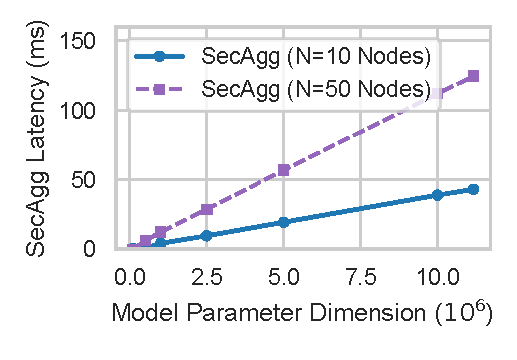
\includegraphics[width=0.48\textwidth]{figures/fig_secagg_overhead.pdf}}
\caption{Execution latency of threshold Secure Aggregation as a function of model parameter dimension, demonstrating efficient key agreement and masking performance.}
\label{fig:secagg_overhead}
\end{figure}

\subsection{Formal Privacy Accounting via R\'enyi Differential Privacy}

While Secure Aggregation protects updates in transit, global model updates can still leak sensitive information across consecutive training rounds~\cite{zhu2019deep, shokri2017membership}. To provide formal privacy guarantees, FedGuard incorporates Differential Privacy (DP) using the Gaussian Mechanism paired with R\'enyi Differential Privacy (RDP) accounting~\cite{abadi2016deep, mironov2017renyi}.

\subsubsection{Gradient Clipping and Noise Addition}
Before transmission, each client bounds the influence of any single record by clipping local update tensors $\Delta_u = \theta_u^{(t)} - \theta^{(t-1)} \in \mathbb{R}^d$ to a maximum $L_2$ norm threshold $C = 1.0$:
\begin{equation}
    \bar{\Delta}_u = \Delta_u \cdot \min\left(1, \, \frac{C}{\|\Delta_u\|_2}\right)
\end{equation}
Zero-mean Gaussian noise scaled by noise multiplier $\sigma = 0.85$ is added to the aggregated update tensor:
\begin{equation}
    \tilde{\Delta} = \sum_{u \in \mathcal{U}} \bar{\Delta}_u + \mathcal{N}\left(0, \, \sigma^2 C^2 \mathbf{I}_d\right)
\end{equation}
where $\mathbf{I}_d$ is the $d \times d$ identity matrix.

\subsubsection{RDP Privacy Budget Composition}
A randomized mechanism $\mathcal{M}$ satisfies $(\alpha, \epsilon_{\text{RDP}})$-R\'enyi Differential Privacy if for any neighboring datasets $D, D'$ differing on a single record, the R\'enyi divergence of order $\alpha > 1$ satisfies:
\begin{equation}
\begin{aligned}
    D_\alpha\big( \mathcal{M}(D) \parallel \mathcal{M}(D') \big) = \frac{1}{\alpha - 1} \ln \mathbb{E}_{x \sim \mathcal{M}(D')} \\
    \times \left[ \left( \frac{\mathcal{M}(D)(x)}{\mathcal{M}(D')(x)} \right)^\alpha \right] \le \epsilon_{\text{RDP}}(\alpha)
\end{aligned}
\end{equation}

For the Gaussian mechanism with scale parameter $\sigma$, the per-round RDP bound is given by $\epsilon_{\text{RDP}}(\alpha) = \frac{\alpha}{2 \sigma^2}$. By the linear composition theorem of RDP, the cumulative privacy loss over $T$ training rounds across order $\alpha$ evaluates to:
\begin{equation}
    \epsilon_{\text{total}}(\alpha) = \sum_{t=1}^{T} \epsilon_{\text{RDP}}^{(t)}(\alpha) = \frac{T \cdot \alpha}{2 \sigma^2}
\end{equation}
To express privacy guarantees in standard $(\epsilon, \delta)$-DP, we convert RDP bounds via optimal dual conversion (Proposition 3 of Balle et al.~\cite{balle2020hypothesis}) at target $\delta = 10^{-5}$:
\begin{equation}
\begin{aligned}
    \epsilon(\delta) = \min_{\alpha > 1} \Big\{ &\frac{T \cdot \alpha}{2 \sigma^2} + \frac{\ln(1/\delta)}{\alpha - 1} \\
    &+ \frac{(\alpha - 1)\ln(1 - 1/\alpha) - \ln \alpha}{\alpha - 1} \Big\}
\end{aligned}
\end{equation}

\begin{figure}[htbp]
\centerline{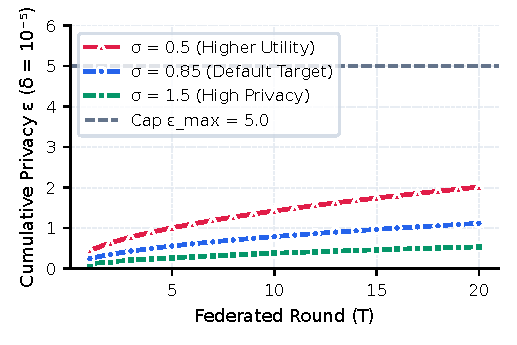
\includegraphics[width=0.48\textwidth]{figures/fig_privacy_budget.pdf}}
\caption{Cumulative differential privacy budget consumption $(\epsilon)$ across federated training rounds for $\delta=10^{-5}, C=1.0, \sigma=0.85$, illustrating dynamic privacy threshold enforcement.}
\label{fig:privacy_budget}
\end{figure}

As shown in Fig.~\ref{fig:privacy_budget}, the RDP accountant tracks cumulative privacy spending in real time. If $\epsilon(\delta)$ exceeds the organization's statutory privacy threshold $\epsilon_{\text{max}} = 5.0$, FedGuard automatically halts training to prevent privacy budget exhaustion.

\subsection{Byzantine-Robust Aggregation under Heterogeneous Data (\texttt{BYZANTINE\_RESILIENT} Mode)}

In active threat environments where malicious clients may transmit poisoned updates~\cite{fang2020local}, FedGuard executes in \texttt{BYZANTINE\_RESILIENT} mode. In this mode, individual update vectors are unmasked to allow coordinate-wise distance metrics and sorting across local datasets exhibiting non-Identically and Independently Distributed (non-IID) characteristics, modeled using a Dirichlet distribution $\operatorname{Dir}(\alpha=0.5)$~\cite{hsu2019measuring, li2020federated}.

FedGuard supports three Byzantine-robust aggregation primitives:
\begin{enumerate}
    \item \textbf{Trimmed Mean:} Let $x_{(1), j} \le x_{(2), j} \le \dots \le x_{(|\mathcal{U}|), j}$ denote the sorted coordinate values along dimension $j \in \{1, \dots, d\}$ across active clients. For trimming fraction $\beta \in [0, 0.5)$~\cite{yin2018byzantine}:
    \begin{equation}
        \tilde{x}_j = \frac{1}{|\mathcal{U}| - 2\lfloor \beta |\mathcal{U}| \rfloor} \sum_{i = \lfloor \beta |\mathcal{U}| \rfloor + 1}^{|\mathcal{U}| - \lfloor \beta |\mathcal{U}| \rfloor} x_{(i), j}
    \end{equation}
    \item \textbf{Coordinate-wise Median:} Each coordinate $j$ of the global update is set to the median value across all reporting clients~\cite{yin2018byzantine}:
    \begin{equation}
        \tilde{x}_j = \operatorname{median}\Big( \{ x_{u, j} \}_{u \in \mathcal{U}} \Big)
    \end{equation}
    \item \textbf{Krum Aggregation:} For each client $i \in \mathcal{U}$, let $S_i \subset \mathcal{U} \setminus \{i\}$ denote the subset of $|\mathcal{U}| - f - 2$ closest updates to $x_i$ in Euclidean $L_2$ distance, where $f < \lfloor \frac{|\mathcal{U}| - 2}{2} \rfloor$ is the upper bound on Byzantine clients~\cite{blanchard2017machine}. Krum selects update vector $x_{k^*}$ where:
    \begin{equation}
        k^* = \arg\min_{i \in \mathcal{U}} \sum_{j \in S_i} \| x_i - x_j \|_2^2
    \end{equation}
\end{enumerate}
By combining robust aggregation rules with non-IID data partitioning ($\alpha=0.5$), FedGuard mitigates sign-flipping and gradient poisoning attacks while preserving global model convergence.
